\documentclass[10pt,fleqn]{article} % Default font size and left-justified equations
\usepackage[%
    pdftitle={Modélisation systèmes multiphysiques : Modélisation linéaire et non linéaire},
    pdfauthor={Xavier Pessoles}]{hyperref}
    
\input{style/new_style}
%%%%%%%%%%%%
% Définition des vecteurs 
%%%%%%%%%%%%

\newcommand{\vect}[1]{\overrightarrow{#1}}
\newcommand{\axe}[2]{\left(#1,\vect{#2}\right)}
\newcommand{\couple}[2]{\left(#1,\vect{#2}\right)}
\newcommand{\angl}[2]{\left(\vect{#1},\vect{#2}\right)}

\newcommand{\rep}[1]{\mathcal{R}_{#1}}
\newcommand{\bas}[1]{\mathcal{B}_{#1}}
\newcommand{\quadruplet}[4]{\left(#1;#2,#3,#4 \right)}
\newcommand{\repere}[4]{\left(#1;\vect{#2},\vect{#3},\vect{#4} \right)}
\newcommand{\base}[3]{\left(\vect{#1},\vect{#2},\vect{#3} \right)}


\newcommand{\vx}[1]{\vect{x_{#1}}}
\newcommand{\vy}[1]{\vect{y_{#1}}}
\newcommand{\vz}[1]{\vect{z_{#1}}}
\newcommand{\vi}[1]{\vect{i_{#1}}}
\newcommand{\vj}[1]{\vect{j_{#1}}}
\newcommand{\vk}[1]{\vect{k_{#1}}}
\newcommand{\vAB}{\vect{AB}}
\newcommand{\vBA}{\vect{BA}}
\newcommand{\vBC}{\vect{BC}}
\newcommand{\vCB}{\vect{CB}}
\newcommand{\vCA}{\vect{CA}}
\newcommand{\vAC}{\vect{AC}}


% d droit pour le calcul différentiel
\newcommand{\dd}{\text{d}}
\newcommand{\deriv}[2]{ \dfrac{ \dd }{\dd t} \left[  #1\right]_{#2}}
\newcommand{\dderiv}[2]{ \dfrac{ \dd^2 }{\dd t^2} \left[  #1\right]_{#2}}

% dérivée
\newcommand{\varphip}{\dot{\varphi}}
\newcommand{\thetap}{\dot{\theta}}
\newcommand{\lambdap}{\dot{\lambda}}
\newcommand{\varphipp}{\ddot{\varphi}}
\newcommand{\thetapp}{\ddot{\theta}}
\newcommand{\lambdapp}{\ddot{\lambda}}



\newcommand{\inertie}[2]{I_{#1}\left( #2\right)}
\newcommand{\matinertie}[7]{
\begin{pmatrix}
#1 & #6 & #5 \\
#6 & #2 & #4 \\
#5 & #4 & #3 \\
\end{pmatrix}_{#7}}
%%%%%%%%%%%%
% Définition des torseurs 
%%%%%%%%%%%%

\newcommand{\ec}[2]{%
\mathcal{E}_c\left(#1/#2\right)}

\newcommand{\pext}[3]{%
\mathcal{P}\left(#1\rightarrow#2/#3\right)}

\newcommand{\pint}[3]{%
\mathcal{P}\left(#1 \stackrel{\text{#3}}{\leftrightarrow} #2\right)}


 \newcommand{\torseur}[1]{%
\left\{{#1}\right\}
}

\newcommand{\torseurcin}[3]{%
\left\{\mathcal{#1} \left(#2/#3 \right) \right\}
}

\newcommand{\torseurci}[2]{%
%\left\{\sigma \left(#1/#2 \right) \right\}
\left\{\mathcal{C} \left(#1/#2 \right) \right\}
}
\newcommand{\torseurdyn}[2]{%
\left\{\mathcal{D} \left(#1/#2 \right) \right\}
}


\newcommand{\torseurstat}[3]{%
\left\{\mathcal{#1} \left(#2\rightarrow #3 \right) \right\}
}


 \newcommand{\torseurc}[8]{%
%\left\{#1 \right\}=
\left\{
{#1}
\right\}
 = 
\left\{%
\begin{array}{cc}%
{#2} & {#5}\\%
{#3} & {#6}\\%
{#4} & {#7}\\%
\end{array}%
\right\}_{#8}%
}

 \newcommand{\torseurcol}[7]{
\left\{%
\begin{array}{cc}%
{#1} & {#4}\\%
{#2} & {#5}\\%
{#3} & {#6}\\%
\end{array}%
\right\}_{#7}%
}

 \newcommand{\torseurl}[3]{%
%\left\{\mathcal{#1}\right\}_{#2}=%
\left\{%
\begin{array}{l}%
{#1} \\%
{#2} %
\end{array}%
\right\}_{#3}%
}

% Vecteur vitesse
\newcommand{\vectv}[3]{%
\vect{V\left( {#1} , {#2}/{#3}\right)}
}

% Vitesse du point
\newcommand{\vectvp}[2]{%
\vect{V\left( {#1} /{#2}\right)}
}

% Vecteur force
\newcommand{\vectf}[2]{%
\vect{R\left( {#1} \rightarrow {#2}\right)}
}

% Vecteur moment stat
\newcommand{\vectm}[3]{%
\vect{\mathcal{M}\left( {#1}, {#2} \rightarrow {#3}\right)}
}




% Vecteur résultante cin
\newcommand{\vectrc}[2]{%
\vect{R_c \left( {#1}/ {#2}\right)}
}
% Vecteur moment cin
\newcommand{\vectmc}[3]{%
\vect{\sigma \left( {#1}, {#2} /{#3}\right)}
}


% Vecteur résultante dyn
\newcommand{\vectrd}[2]{%
\vect{R_d \left( {#1}/ {#2}\right)}
}
% Vecteur moment dyn
\newcommand{\vectmd}[3]{%
\vect{\delta \left( {#1}, {#2} /{#3}\right)}
}

% Vecteur accélération
 \newcommand{\vectg}[3]{%
\vect{\Gamma \left( {#1}, {#2}/{#3}\right)}
}
% Vecteur accélération du point
 \newcommand{\vectgp}[2]{%
\vect{\Gamma \left( {#1}/{#2}\right)}
}

% Vecteur omega
 \newcommand{\vecto}[2]{%
\vect{\Omega\left( {#1}/{#2}\right)}
}
% }$$\left\{\mathcal{#1} \right\}_{#2} =%
% \left\{%
% \begin{array}{c}%
%  #3 \\%
%  #4 %
% \end{array}%
% \right\}_{#5}}

%Varignon dynamique
 \newcommand{\babard}[4]{%
\vectmd{#1}{#3}{#4}=\vectmd{#2}{#3}{#4}+\vect{#1#2}\wedge \vectrd{#3}{#4}
}

%Varignon cinématique
 \newcommand{\babarv}[4]{%
\vectv{#1}{#3}{#4}=\vectv{#2}{#3}{#4}+\vect{#1#2}\wedge \vecto{#3}{#4}
}

%% SLCI
% Ordre 1
\newcommand{\ordreun}{\dfrac{K}{1+\tau p}}

\newcommand{\ordreunopt}[2]{\dfrac{#1}{1+#2 p}}
% Ordre 2
\newcommand{\ordredeux}{\dfrac{K}{1+\dfrac{2\xi}{\omega_0}p+\dfrac{p^2}{\omega_0^2}}}

% MCC
\newcommand{\mccel}{U(t)=E(t)+RI(t)+L\dfrac{\dd i(t)}{\dd t}}
%\newcommand{\mccmeca}{J \dfrac{\dd \omega(t)}{\dd t}=C }




%Binaire, octal, hexa
\newcommand{\hex}[1]{\underline{\text{\texttt{#1}}}_{16}}
\newcommand{\oct}[1]{\underline{\text{\texttt{#1}}}_{8}}
\newcommand{\bin}[1]{\underline{\text{\texttt{#1}}}_{2}}


% Fonctions et systèmes
\usepackage{multicol}
\usepackage{standalone}
\standaloneconfig{mode=buildnew}
\usepackage{siunitx}
\usepackage{wrapfig}
\fichetrue

%\fichefalse

%\proftrue
%\proffalse

\tdtrue
%\tdfalse

\courstrue
\coursfalse

\def\discipline{Sciences \\Industrielles de \\ l'Ingénieur}
\def\xxtete{Sciences Industrielles de l'Ingénieur}

\def\classe{PSI$\star$}
\def\xxnumpartie{}%\textsf{Cy.  \& 5}}
\def\xxpartie{Devoir Surveille 6}


\def\xxnumchapitre{17 Février 2020 \vspace{.2cm}}
\def\xxchapitre{\hspace{.12cm} Modélisation multiphysique}


\def\xxtitreexo{\noindent Chariot élévateur de bateaux}%Motorisation du moteur Haibike}
\def\xxsourceexo{\hspace{.2cm} X--ENS PSI 2012}


\def\xxposongletx{2}
\def\xxposonglettext{1.45}
\def\xxposonglety{20}
%\def\xxonglet{Part. 1 -- Ch. 3}
\def\xxonglet{Cy. 4 \& 5}

\def\xxactivite{DS 6}
\def\xxauteur{\textsl{Xavier Pessoles}}

\def\xxcompetences{%
\textsl{%
%\textbf{Savoirs et compétences :}\\
%Les sources sont associées par un \emph{hacheur série}. La détermination des grandeurs électriques associées à ce montage permet de conclure vis à vis du cahier des charges.
%\noindent \textbf{Résoudre :} à partir des modèles retenus :
%\begin{itemize}[label=\ding{112},font=\color{ocre}] 
%\item choisir une méthode de résolution analytique, graphique, numérique;
%\item mettre en \oe{}uvre une méthode de résolution.
%\end{itemize}
%\begin{itemize}[label=\ding{112},font=\color{ocre}] 
%\item \textit{Rés -- C1.1 :} Loi entrée sortie géométrique et cinématique -- Fermeture géométrique.
%\end{itemize}
%
%\noindent \textit{Mod2 -- C4.1 :} Représentation par schéma-blocs.
}}

\def\xxfigures{
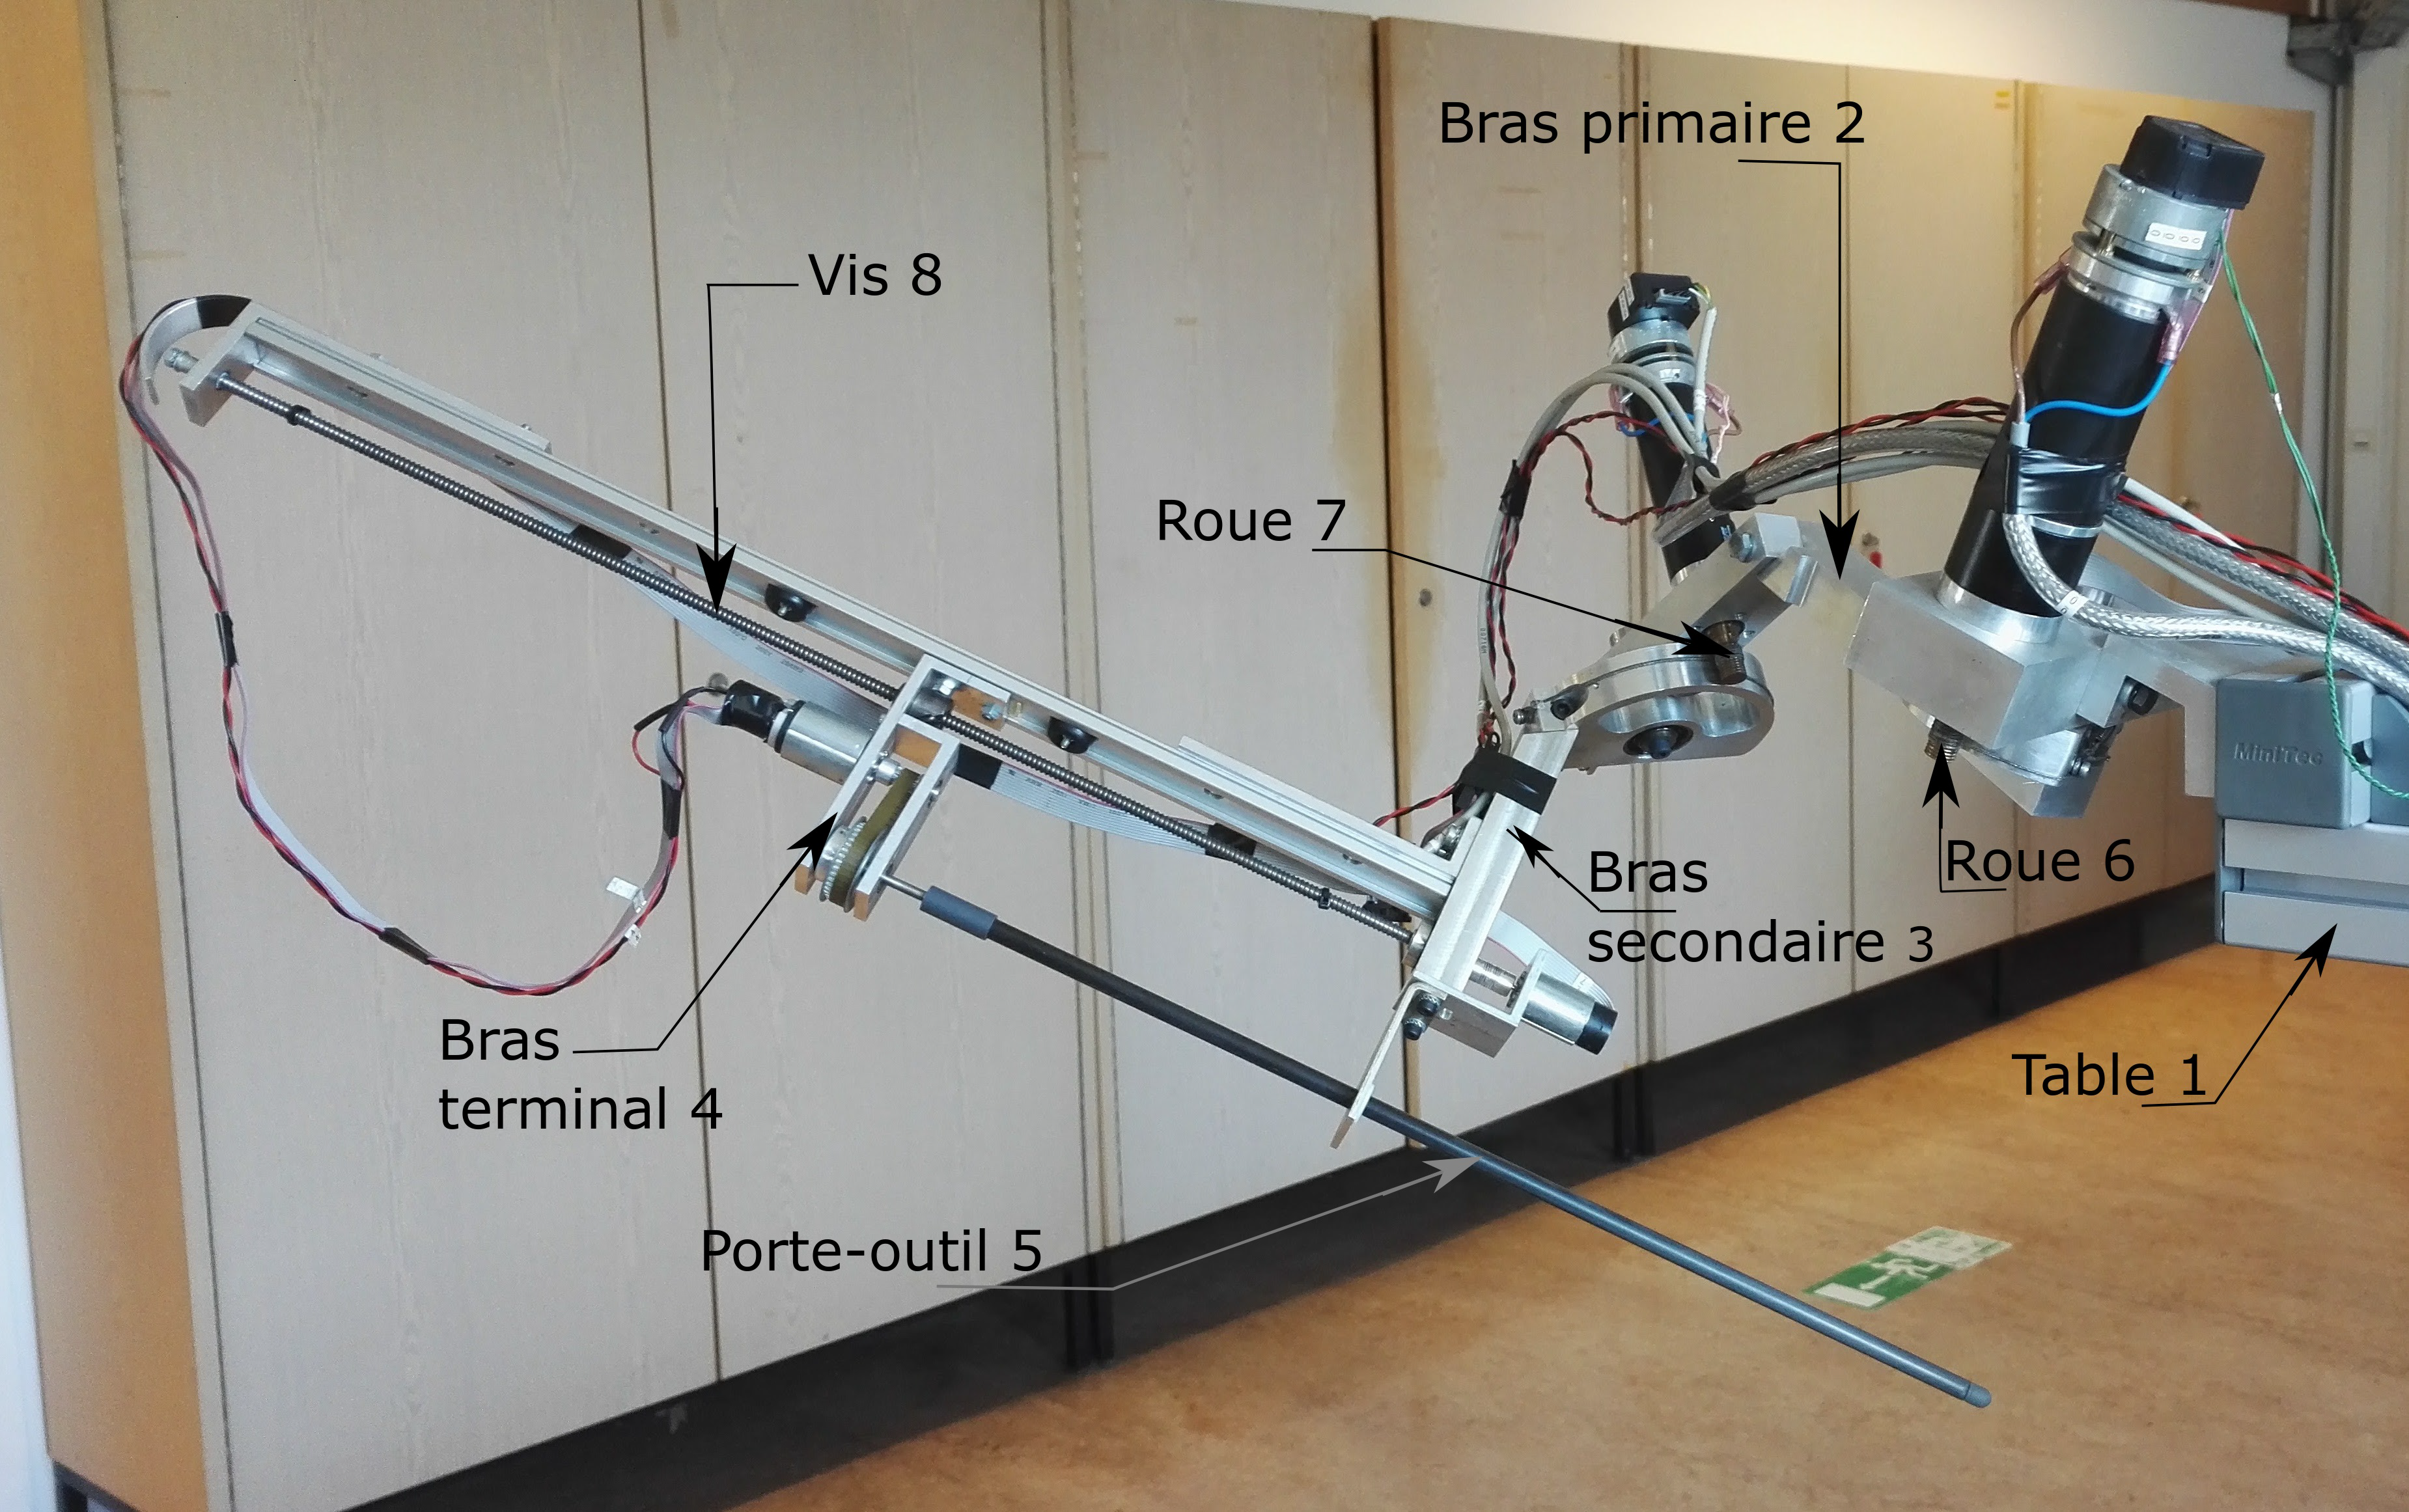
\includegraphics[width=.9\linewidth]{images/fig_00}
}%figues de la page de garde


\def\xxpied{%
%Cycle 01 -- Modéliser le comportement des systèmes multiphysiques\\
\xxactivite%
}

\setcounter{secnumdepth}{5}
%---------------------------------------------------------------------------

\usepackage{pgfplots}
\begin{document}
%\defimages{images}
%\chapterimage{png/Fond_Cin}
\input{style/new_pagegarde}
\vspace{7cm}
\pagestyle{fancy}
\thispagestyle{plain}

\def\columnseprulecolor{\color{ocre}}
\setlength{\columnseprule}{0.4pt} 

%\defimages2{images}

%\begin{multicols}{2}
\section*{Mise en situation}
%\subsection{Présentation générale}

Le stockage des bateaux dans des « ports à sec » offre une solution alternative à la saturation des ports de plaisance tout en limitant fortement les contraintes d’entretien et de maintenance. Les bateaux sont stockés dans des casiers et sont mis à l’eau et rangés grâce à des chariots élévateurs à bateaux. L’objet de cette étude, représenté sur la Figure 1, est l’un de ces chariots élévateurs qui assurent les opérations de « sortie de l’eau -- dépose dans le casier » ou « sortie du casier -- mise à l’eau ». Compte tenu du nombre important de bateaux stockés, la prestation principale doit satisfaire l’impatience des plaisanciers. Le schéma de la Figure 2 décrit cette prestation.

\begin{center}
\begin{tabular}{ccc}
\includegraphics[height=4cm]{images/fig_01_a} &&
\includegraphics[height=4cm]{images/fig_01_b}
\end{tabular}

%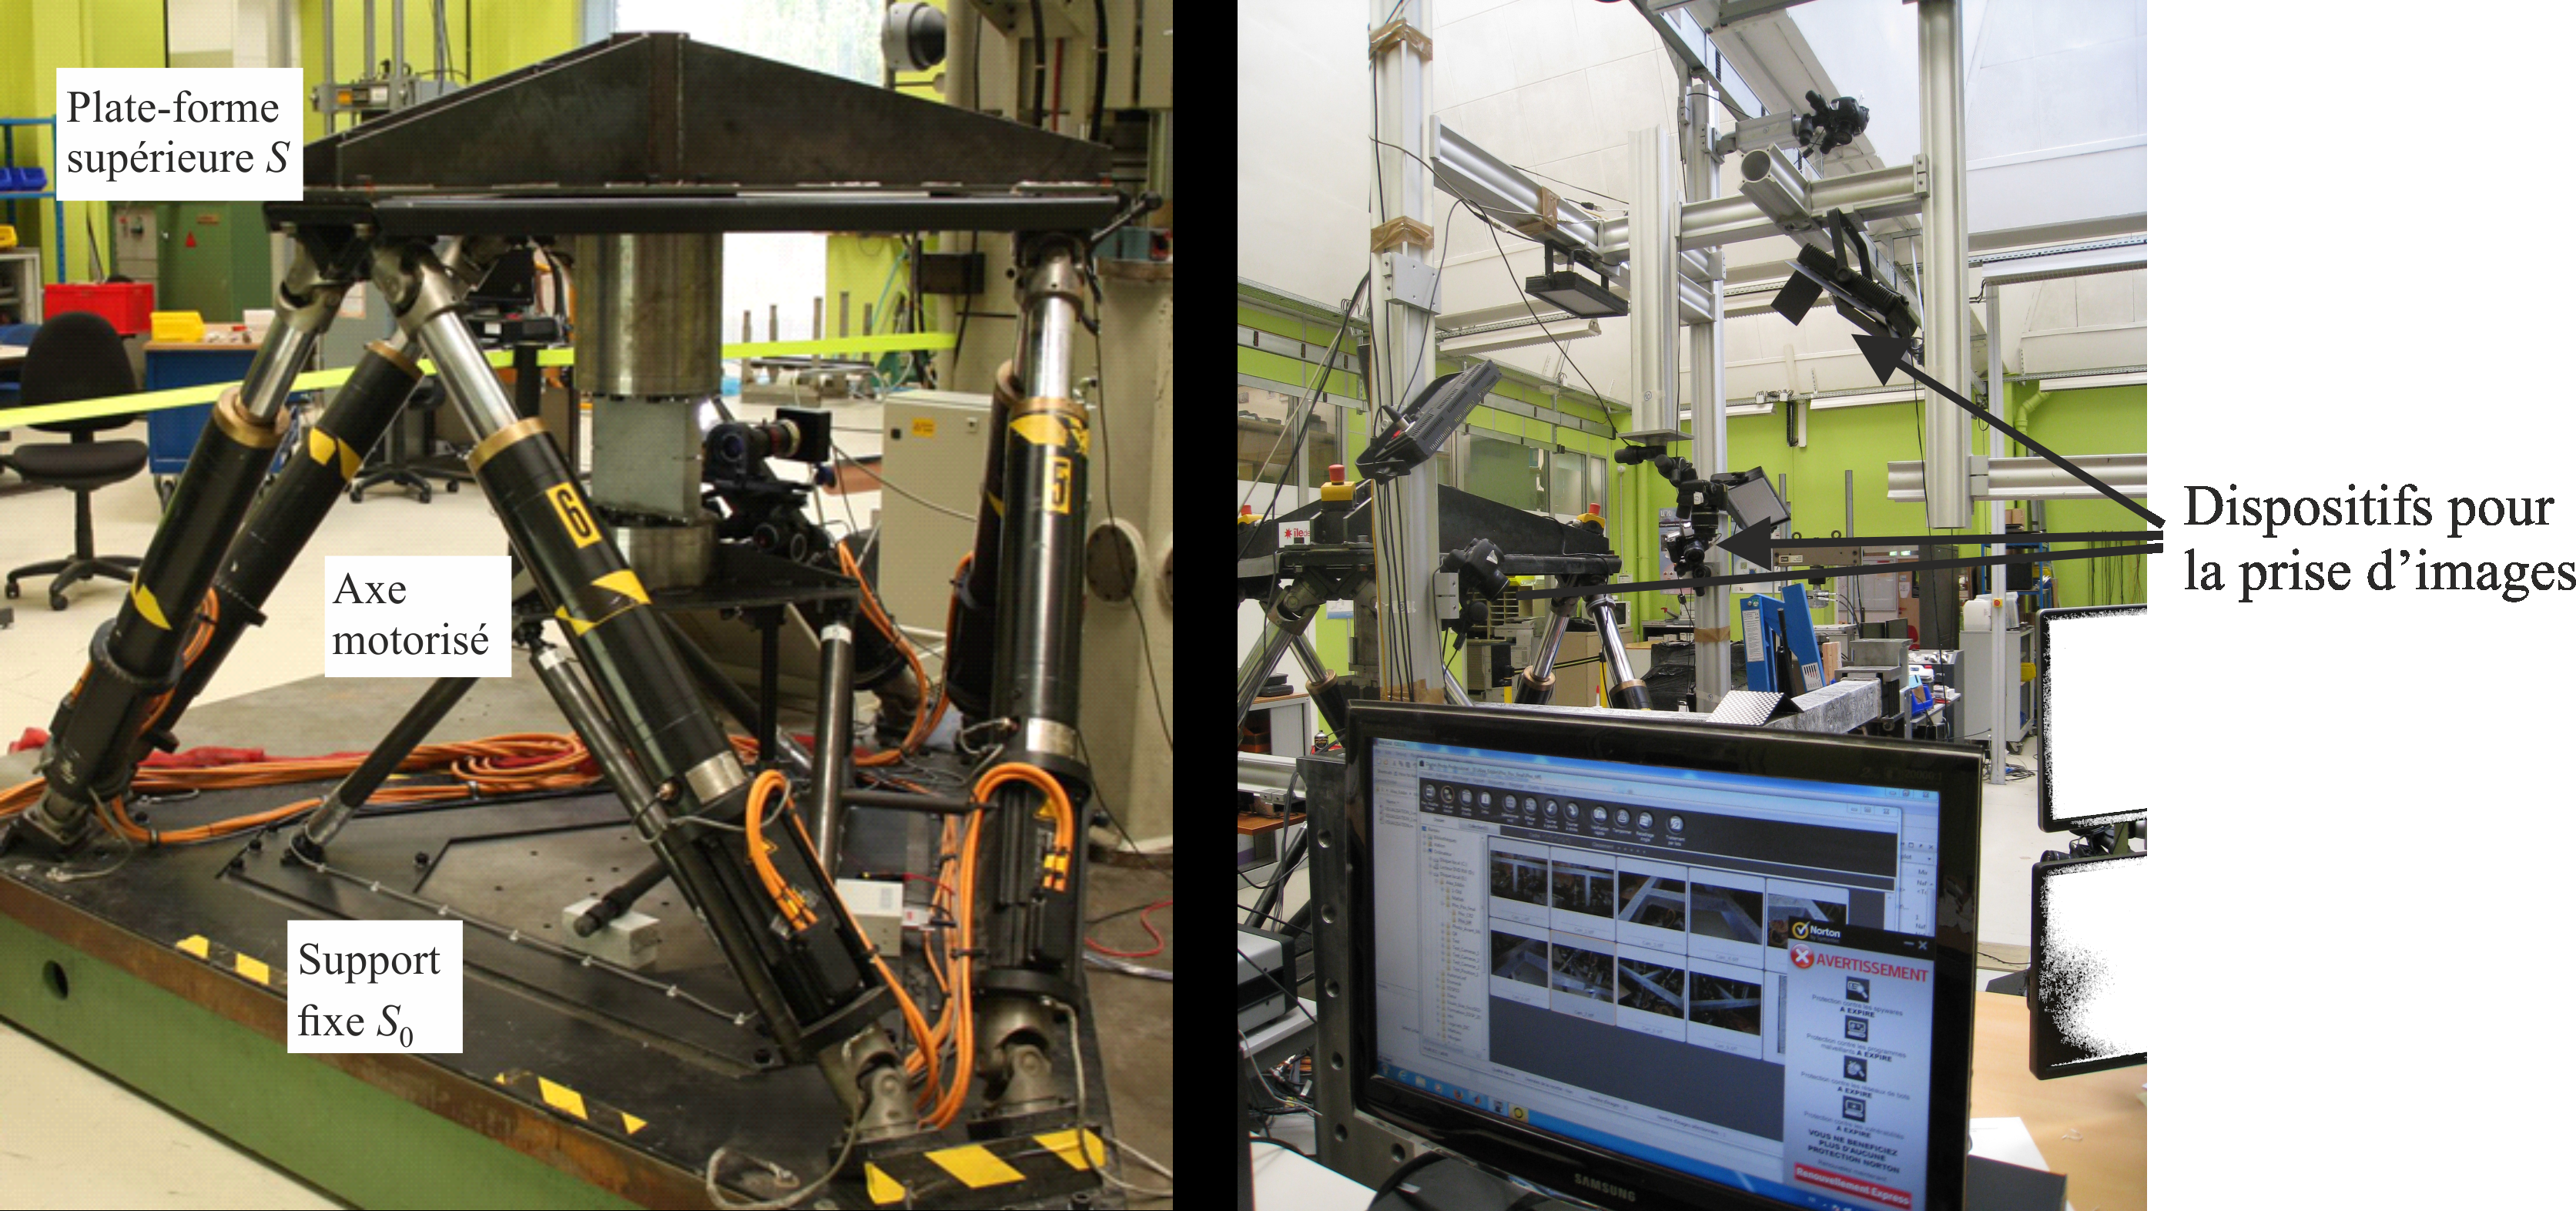
\includegraphics[width=1.\linewidth]{images/fig_01}
\textit{Figure 1}
\end{center}


\begin{center}
\includegraphics[width=.8\linewidth]{images/fig_02}

\textit{Figure 2}
\end{center}

Ce type de chariot élévateur, représenté sur la Figure 3, permet la manutention de bateaux de \SI{3000}{kg} à une hauteur de \SI{8}{m}. Il est principalement constitué :
\begin{itemize}
\item du chariot qui assure le déplacement de l’ensemble et apporte la puissance pour la préhension et le levage ;
\item du tablier, constitué du mât et des fourches, qui permet la préhension et la dépose du bateau.
\end{itemize}



\begin{center}
\includegraphics[width=.8\linewidth]{images/fig_03}

\textit{Figure 3}
\end{center}


Le trajet du chariot, représenté sur la Figure 4, est imposé par la disposition des casiers par rapport au quai de mise à l’eau. Afin d’optimiser la fréquence de mise à l’eau des bateaux, tout en garantissant les conditions de sécurité, il est nécessaire d’optimiser le temps de déplacement du chariot en ligne droite, en virage ou en freinage. Le principal danger auquel est confronté le conducteur est le basculement du chariot.
\begin{obj}
L’objectif de l’étude est de valider les fonctions techniques caractérisant la spécificité du tablier et de mettre en évidence la nécessité des dispositifs de sécurité qui permettent au chariot d’assurer une cadence optimale dans les phases de vie considérées, en lui permettant de se déplacer à des vitesses élevées.
\end{obj}


\begin{center}
\includegraphics[width=.8\linewidth]{images/fig_04}

\textit{Figure 4}
\end{center}



L’étude comprend trois parties :
\begin{itemize}
\item la partie I a pour objet l’analyse de la préhension et de la dépose du bateau ;
\item la partie II a pour objet l’analyse de la transmission du chariot et la validation de ses performances en déplacement ;
\item la partie III a pour objet l’analyse de la stabilité du chariot élévateur lors de la phase de déplacement et la validation de la cadence de mise à l’eau des bateaux.
\end{itemize}

Une partie du cahier des charges, pour un regroupement des phases de vie « chargement --déplacement-mise à l’eau du bateau » est donnée par la Figure 5.


\begin{center}
\includegraphics[width=.5\linewidth]{images/fig_05a}

\includegraphics[width=1.\linewidth]{images/fig_05}

\textit{Figure 5}
\end{center}


\section{Partie 1 : Validation de l'exigence 1}
L’objet de cette partie est de valider les critères des exigences 1 et 3 et l’aptitude du tablier à remplir toutes les fonctions techniques concernant la préhension et la dépose du bateau. L’annexe1 présente les mouvements possibles du tablier qui permettent d’assurer la préhension du bateau. L'exigence 1 est déclinée par fonctions dans l'annexe 2. Un schéma cinématique du tablier est disponible en annexe 3. La caractérisation partielle des exigences 1 et 3 est donnée sur la Figure 6.

\begin{center}
\includegraphics[width=1.\linewidth]{images/fig_06}

\textit{Figure 6}
\end{center}

\subsection{Phase d'ouverture des fourches}
Le modèle d’étude retenu pour cette partie est donné en ANNEXE 3.
L’analyse qui suit porte sur le mécanisme d’ouverture des fourches constitué des pièces T6,T7,T8,T9,T10 et T11. Le chariot est immobile, les mécanismes de basculement, de levage et de déplacement latéral du tablier sont inactifs.

La sortie de la tige du vérin T11 entraîne la rotation de la fourche droite T8 autour de l’axe $\axe{C}{x_{T8}}$. Le mouvement d’ouverture est transmis par l’intermédiaire de la barre de renvoi T9 à la fourche gauche T7 qui est entraînée en rotation autour de l’axe $\axe{F}{x_{T6}}$. On obtient ainsi le mouvement d’ouverture des fourches.

On définit les repères suivants :
\begin{itemize}
\item $\mathcal{R}_0=\repere{O_0}{x_0}{y_0}{z_0}$ est un référentiel galiléen lié à la route. $\vect{z_0}$ est vertical ascendant;
\item $\mathcal{R}_{T6}=\repere{F}{x_{T6}}{y_{T6}}{z_{T6}}$  est un repère supposé galiléen dans les conditions de l’étude, lié à la pièce T6 de masse $m_{T6}$;
\item $\mathcal{R}_{T7}=\repere{G_{T7}}{x_{T7}}{y_{T7}}{z_{T7}}$  est un repère lié à la fourche gauche T7 de masse $m_{T7}$. $G_{T7}$ est le centre de gravité du solide T7, $\vect{x_{T6}}=\vect{x_{T7}}$ et $\angl{{y_{T6}}}{{y_{T7}}}=\angl{{z_{T6}}}{{z_{T7}}}=\theta_2$;
\item $\mathcal{R}_{T8}=\repere{G_{T8}}{x_{T8}}{y_{T8}}{z_{T8}}$  est un repère lié à la fourche droite T8 de masse $m_{T8}$. $G_{T8}$ est le centre de gravité du solide T8, $\vect{x_{T6}}=\vect{x_{T8}}$ et $\angl{{y_{T6}}}{{y_{T8}}}=\angl{{z_{T6}}}{{z_{T8}}}=\theta_1$;
\item $\mathcal{R}_{T9}=\repere{D}{x_{T9}}{y_{T9}}{z_{T9}}$  est un repère lié à la barre de renvoi T9, $\vect{x_{T6}}=\vect{x_{T9}}$ et $\angl{{y_{T6}}}{{y_{T9}}}\angl{{z_{T6}}}{{z_{T9}}}=\theta_4$. La masse du solide T9 sera négligée;
\item $\mathcal{R}_{T10}=\repere{A}{x_{T10}}{y_{T10}}{z_{T10}}$  est un repère lié au corps du vérin T10, ${x_{T6}}={x_{T10}}$ et $\angl{{y_{T6}}}{{y_{T10}}}\angl{{z_{T6}}}{{z_{T10}}}=\theta_3$, la position relative des solides T9 et T10 est donnée par $\vect{BA}=\mu\vect{z_{T10}}$. Les masses des solides T10 et T11 seront négligées.
\end{itemize}
Pour la suite de l'étude, le basculement est en position neutre, les mâts inférieur T3 et supérieur T4 ainsi que le vecteur $\vect{z_{T6}}$ sont donc verticaux. 




\subparagraph{}
\textit{Écrire, sans les projeter, les équations vectorielles qui établissent les relations entre $\theta_1$ ,$\theta_2$ ,$\theta_3$ ,$\theta_4$ et $\mu$ et justifier le choix d’un unique actionneur pour commander le mécanisme d’ouverture.}

La position de référence du mécanisme est définie telle que à $t=\SI{0}{s}$ : $\theta_1(0)=\SI{0}{\degres}$,  $\theta_2(0)=\SI{0}{\degres}$ et $\mu(0)=\SI{777}{mm}$.


\subparagraph{}
\textit{Dans ces conditions, donner l’expression de la longueur $f$ de la barre de renvoi permettant de valider la position de référence en fonction de $a$, $b$, $c$, $d$ et $e$.}

Les courbes en ANNEXE 4 donnent l’évolution des différents paramètres en fonction du temps pour un cycle d’ouverture. L’instant initial de la simulation correspond à la position de référence.
On admet que la distance $c_{\text{v\'erin}}$ est la distance parcourue par la tige du vérin par rapport au corps du vérin. On considère que  $c_{\text{v\'erin}}=0$  correspond à la position de référence du mécanisme.

\subparagraph{}
\textit{En analysant ces courbes, donner la valeur de la course $c_{\text{v\'erin}}$ du vérin 
permettant de valider l'exigence 1.4.2.2. L'exigence 1.4.3 est-elle validée ? Justifier.}


La barre de renvoi T9 transmet le mouvement de la fourche droite à la fourche gauche. Le fonctionnement idéal du mécanisme devrait permettre une ouverture rigoureusement identique des deux fourches durant le cycle d’ouverture.

\subparagraph{}
\textit{Écrire la relation entre $\theta_1$ et $\theta_2$ qui assure une ouverture angulaire identique des deux fourches. Le critère 1.4.4 est-il validé ? Justifier. Quelle flexibilité en \% faut-il négocier sur ce critère afin d’éviter toute modification sur le mécanisme ? Donner un argument permettant de négocier cette flexibilité.}


Le choix du vérin d’ouverture T10 -- T11 nécessite une étude préalable des efforts développés par l’actionneur durant la phase d’ouverture. Compte tenu des faibles accélérations des différents solides, les effets dynamiques seront négligés.

Le torseur modélisant l’action mécanique du solide $T_i$ sur le solide $T_j$ est noté :
$$
\torseurstat{T}{T_i}{T_j}
=
\torseurl{
\vectf{T_i}{T_j}
}{
\vectm{M}{T_i}{T_j}
}{M}
=
\torseurcol{X_{T_i \to T_j}}{Y_{T_i \to T_j}}{Z_{T_i \to T_j}}{L_{T_i \to T_j}}{M_{T_i \to T_j}}{N_{T_i \to T_j}}{M,\mathcal{R}_{Tk}}
 \quad \text{au point }M\text{ dans le repère de projection }\mathcal{R}_{Tk}.
$$

\subparagraph{}
\textit{En analysant la chaîne de solides $\left\{T_6, T_7, T_8, T_9, T_{10}, T_{11} \right\}$, montrer qu’il est possible de déterminer le torseur $\torseurstat{T}{T_{11}}{T_{8}}$ représentant l’action mécanique exercée par le vérin $T_{11}$ sur la fourche $T_{8}$. Les différentes étapes de l’analyse seront détaillées. Le calcul des éléments de réduction de $\torseurstat{T}{T_{11}}{T_{8}}$ n’est pas demandé.}



La courbe de la figure 7 donne l’évolution de la résultante $\vectf{T_{11}}{T_{8}}$ en fonction de la course $c_{\text{v\'erin}}$ du vérin $T_{10}$ -- $T_{11}$.

\begin{center}
\includegraphics[width=.65\linewidth]{images/fig_07}

\textit{Figure 7}
\end{center}

\subparagraph{}
\textit{Quelle est la valeur de $||\vectf{T_{11}}{T_{8}}||$ à retenir pour le dimensionnement du vérin $T_{10}$ -- $T_{11}$ dans le cas d’une amplitude d’ouverture conforme à celle préconisée par le cahier des charges.}

\subsection{Phase de fermeture des fourches}
Lors de la phase de fermeture, il est nécessaire de limiter la vitesse des fourches afin de permettre au conducteur de contrôler leurs positions et de limiter la vitesse d’impact en cas de contact avec la coque du bateau. Il faut également limiter l’effort de serrage des fourches sur le bateau en cas de mauvaise manipulation du conducteur (les fourches doivent normalement passer sous la coque du bateau).

Un régulateur de débit proportionnel et un limiteur de pression sont installés dans le circuit hydraulique d’alimentation du vérin afin de garantir ces conditions de fonctionnement.


\subparagraph{}
\textit{Exprimer $\dot{\theta_1}(t) = \dfrac{\dd \theta_1(t)}{\dd t}$  en fonction de $\mu$, ${\theta_1}$ et $\dot{\mu}$.}


L’exploitation de la relation établie nous permet de tracer le réseau de courbes de la Figure 8 qui donne la variation de $ \dfrac{\dd \theta_1(t)}{\dd t}$ pour différentes valeurs de $\dot{\mu}$(vitesse de rentrée de la tige du vérin $T_{10}$-- $T_{11}$). Les valeurs de $\dot{\mu}$ considérées sont : \SI{0,05}{m/s}, \SI{0,1}{m/s}, \SI{0,15}{m/s} et \SI{0,2}{m/s}.
Pour chaque courbe, la position de départ correspond aux fourches complètement ouvertes et la position de fin correspond à la position de référence.


\begin{center}
\includegraphics[width=.65\linewidth]{images/fig_08}

\textit{Figure 8}
\end{center}


Le circuit hydraulique d’alimentation du vérin est donné sur le document réponse DR 1.
La section de la chambre du vérin $T_{10}$ -- $T_{11}$ est $S_{\text{v\'erin}}=1,3\times10^{-3}\,\text{m}^2$.

\subparagraph{}
\textit{Sur le document réponse DR 1, pour le mouvement de fermeture, indiquer par des flèches le sens de circulation de l’huile dans les canalisations, le sens du déplacement de la tige du vérin et mettre en place le limiteur de pression et le régulateur de débit dans le circuit hydraulique.}


\subparagraph{}
\textit{Quelle doit être la valeur de réglage de la consigne du régulateur de débit proportionnel permettant d’assurer la validation simultanée des exigences 1.4.2.1 et 1.4.3 ? Le raisonnement ne prendra en compte que les 4 valeurs de $\dot{\mu}$ proposées Figure 8.}


\subsection{Phase de levage}
Dans cette partie, on considère que le chariot est à l’arrêt et que le levage est le seul mouvement actif. Le modèle retenu pour cette étude est le schéma de principe de la Figure 9. En raison de la symétrie du tablier par rapport à son plan médian vertical, le modèle d’étude peut se ramener à un système comprenant un seul vérin, une seule chaîne et une seule poulie. L’adaptation des caractéristiques cinétiques des différents solides est déjà prise en compte dans les données fournies dans le sujet afin d’assurer la cohérence entre le système réel et la modélisation choisie.

L’actionneur est un vérin hydraulique dont le corps est en liaison encastrement avec le mât inférieur. La tige est solidaire du mât supérieur. Le levage de l’ensemble $S=\left\{T_5,T_6,T_7,T_8,T_9,T_{10},T_{11}\right\}$ est obtenu à l’aide d’une chaîne présentant un point d’ancrage sur le mât inférieur et un point d’ancrage sur l’ensemble $S$. Cette chaîne roule sans glisser sur le pignon $T_{12}$ qui est en liaison pivot par rapport au mât supérieur.

Le bateau étant à l’arrêt en position basse, le conducteur actionne le levage du bateau.
L’effort de poussée fourni par le vérin est $F_V$ (considéré comme constant). 
On note $I_{T12}$ le moment d’inertie de la poulie $T_{12}$ par rapport à son axe de rotation, $R_{T12}$ son rayon. Sa masse est négligée.
Les masses des différents solides sont rappelées dans le tableau ci-dessous :
\begin{center}
\begin{tabular}{|l|c|}
\hline 
Solide & Masse \\ \hline
Ensemble $S$ & $m_S$ \\ \hline
 Bateau $B$ & $m_B$ \\ \hline
 Mât inférieur $T_3$ & $m_{T3}$ \\ \hline
 Mât supérieur $T_4$ & $m_{T4}$ \\ \hline
 Chaîne $C$ & Masse négligée \\ \hline
\end{tabular}
\end{center}

Les liaisons sont parfaites. La chaîne est non dissipative. Le repère $\mathcal{R}_{T3}$ peut être considéré comme un référentiel galiléen pour les conditions de l’étude. Les axes $\vect{z_{T3}}$ et  $\vect{z_{0}}$ sont confondus pour les conditions de l’étude.

\begin{center}
\includegraphics[width=.65\linewidth]{images/fig_09}

\textit{Figure 9}
\end{center}


\subparagraph{}
\textit{En utilisant le théorème de l'énergie cinétique (énergie - puissance) appliqué à l'ensemble \{Bateau, S, Chaîne, $T_{12}$, $T_4$\}, déterminer l’accélération galiléenne du bateau en fonction de l’effort fourni par le vérin et des caractéristiques du système. Expliquer qualitativement comment cette valeur peut permettre de valider l'exigence 1.1.3.}

\subsection{Phase de déplacement}
La zone de stockage des bateaux se situe nécessairement à une altitude supérieure à celle du quai de déchargement. Afin d’éviter le glissement du bateau lorsque le chariot descend une pente, un dispositif permet de maintenir les fourches horizontales durant le déplacement. Lors d’une phase de décélération, les fourches sont automatiquement inclinées vers l’arrière pour éviter le glissement du bateau. Ce mouvement, de faible amplitude, est assuré par l’asservissement des vérins d’inclinaison du tablier $T_1$, $T_2$ et $T_1’$, $T_2’$. Ce dispositif présente l’avantage de prendre en charge de manière entièrement automatisée l’un des mouvements du tablier. Le conducteur peut alors charger et mettre à l’eau le bateau sans avoir à gérer manuellement le mouvement d’inclinaison.

La Figure 10 permet de définir :
\begin{itemize}
\item l'angle de basculement $\alpha=\left(\vect{z_1},\vect{z_{T3}}\right)$;
\item l'angle de basculement $\delta=\left(\vect{z_0},\vect{z_{1}}\right)$;
\item l'angle à asservir $\varphi=\angl{z_0}{z_{T3}} = \alpha + \delta$.
\end{itemize}



\begin{center}
\includegraphics[width=.8\linewidth]{images/fig_10}

\textit{Figure 10}
\end{center}
%
%Les performances de l'asservissement sont données dans la Figure 11.
%
%
%\begin{center}
%\begin{tabular}{|l|l|}
%\hline 
%Performances attendues de l'asservissement & Essart statique nul \\ \hline
%Précision & Écart statique nul \\ \hline
%Rapidité & $T_{5\,\%} < \SI{0,9}{s}$ \\ \hline
%Amortissement & Pas de dépassement\\ \hline
%Stabilité & Marge de phase \SI{35}{\degres} \\
% & Marge de gain : \SI{10}{dB} \\ \hline
%\end{tabular}
%
%\textit{Figure 11}
%\end{center}
%
%
Le mouvement de basculement est obtenu à l’aide de deux vérins. Compte tenu des considérations de symétrie, l’étude de l’asservissement sera ramenée à l’étude d’un seul vérin et d’une seule servovalve.
Le schéma-blocs du modèle retenu est représenté sur la Figure 12, il est constitué (entre autre) de :
\begin{itemize}
%\item un correcteur dont les caractéristiques seront définies dans la suite du sujet;
%\item un convertisseur qui génère le courant $i(t)$ à partir de la tension de commande $u_c(t)$ obtenue en sortie; 
%\item une servovalve qui délivre un débit volumique d’huile $q_v(t)$ que l’on souhaite proportionnel au courant d’entrée $i(t)$;
%\item un vérin hydraulique ;
\item un inclinomètre monté sur le chariot qui indique l’inclinaison du chariot par rapport à l’horizontale $\delta(t) = \angl{z_0}{z_1}$ (inclinaison de la pente sur laquelle circule le chariot) ; 
\item un capteur angulaire qui indique l’angle de rotation entre les fourches et le chariot $\alpha(t) = \angl{z_1}{z_{T3}}$;
\item un accéléromètre monté sur le chariot qui indique la décélération $\Gamma_{\text{d\'ec}}(t)$ du chariot lors des phases de freinage. Cette information permet, à partir d’un générateur de consigne, d’élaborer la consigne $\varphi_{\text{d\'ec}}$ qui représente l’angle de basculement arrière à imposer aux fourches afin de limiter les risques de glissement du bateau lors de la décélération ;
\item $\varphi(t) = \angl{z_0}{z_{T3}}=\alpha(t)+\delta(t)$ est la grandeur qui sera asservie selon le schéma-blocs de la Figure 12.
\end{itemize}
%
%
\begin{center}
\includegraphics[width=1.\linewidth]{images/fig_12}
\textit{Figure 12}
\end{center}

\subparagraph{}
\textit{Quand le chariot circule à vitesse constante, quelle est la valeur de l’angle $\varphi(t)$ qui permet d’assurer le maintien de l’horizontalité des fourches ? Justifier.}
%
%\subsubsection*{Modèle de connaissance du comportement dynamique du vérin}
%
%\begin{center}
%\includegraphics[width=.35\linewidth]{images/img_01}
%\end{center}
%
%On a : 
%\begin{itemize}
%\item $\lambda(t)$ : déplacement de la tige du vérin par rapport à la position neutre (mât du tablier vertical);
%\item $p(t)$ : différence de pression entre la chambre 1 et la chambre 2;
%\item $Q(t)$ : débit entraînant le déplacement de la tige du vérin;
%\item $S$ : section utile du vérin;
%\item $V_0$ : volume des chambres 1 et 2 quand la tige du vérin est en position neutre;
%\item $B$ : module de compressibilité du fluide.
%\end{itemize}
%
%On admet que la relation suivante qui lie $Q(t)$ et $p(t)$ : 
%$$
%Q(t)=S\dfrac{\dd \lambda(t)}{\dd t} + \dfrac{V_0}{2B} \dfrac{\dd p(t)}{\dd t}.
%$$


\subsubsection*{Modèle de connaissance du comportement dynamique des fourches}

Nous considérons dans cette partie que le seul mouvement actif est le basculement.
L’objectif est d’obtenir un modèle dynamique du mécanisme de basculement à partir de la modélisation plane proposée sur la Figure 13.

Les solides pris en compte pour l’étude sont :
\begin{itemize}
\item l'ensemble $S_2=\left\{ T_3, T_4, T_5, T_6, T_7, T_8, T_9, T_{10},  T_{11}\right\}$ en liaison pivot d’axe $\axe{O_1}{y_0}$ l’ensemble par rapport au chariot 1 de centre de gravité $G_{S_2}$. Le moment d’inertie de l’ensemble $S_2$ par rapport à l’axe $\left(O_1,\vect{y_1}\right)$ sera noté $J_{S2}$ et sa masse $m_{S2}$. La liaison pivot entre l’ensemble $S_2$ et le chariot génère un couple résistant $\vect{C_{\mu}}=-\mu\dot{\alpha} \vect{y_0}$. On a $\vect{O_1G_{S_2}}=\begin{pmatrix} x_{G_{S_2}} \\ 0 \\ z_{G_{S_2}} \end{pmatrix}_{\mathcal{R}_{T3}}$;
\item un vérin équivalent $V=\left\{T_1,T_2\right\}$ dont la tige est en liaison pivot d’axe $\axe{A_1}{{y_0}}$ par rapport au chariot 1 et le corps en liaison pivot d’axe $\axe{B_1}{y_0}$ par rapport à l’ensemble $S_2$. La masse et l’inertie du vérin sont négligées. Le vérin développe un effort au cours du mouvement qui sera noté $\vect{F_V}=p(t)S\vect{z_{T2}}$ où $p(t)$ est la différence de pression entre les deux chambres du vérin.
\end{itemize}

On pose $\vect{A_1B_1} = \left( \lambda_0 + \lambda\right)\vect{z_{T2}}$. Le paramétrage est tel que si $\alpha=0$ alors $\lambda=0$. 


\begin{center}
\includegraphics[width=.8\linewidth]{images/fig_13}

\textit{Figure 13}
\end{center}

Une simulation a permis de tracer la courbe qui donne $\alpha(t)$ en fonction de $\lambda(t)$ sur la plage de variation de $\alpha(t)$ qui correspond au mouvement de basculement. L’analyse de cette courbe nous permet d’approximer une relation linéaire entre $\alpha(t)$ et $\lambda(t)$ de la forme $\alpha(t)=k\lambda(t)$ où $k$ est une constante.


\subparagraph{}
\textit{En appliquant le théorème de l’énergie-puissance et en admettant que l’angle $\alpha$ est petit, montrer que $\alpha(t)$ et $p(t)$ sont liés par l’équation différentielle suivante et exprimer $J_{eq}$ :}
$$
J_{eq}\ddot{\alpha}(t)+\mu \dot{\alpha}(t) = \dfrac{Sp(t)}{k}+m_{S_2}gx_{G_{S_2}}.
$$

%\subparagraph{}
%\textit{Montrer que le comportement du vérin peut, dans ces conditions, être modélisé par le schéma-blocs Figure 14. Donner alors les expressions des fonctions de transfert $A(p)$, $B(p)$, $C(p)$ et $D(p)$. Exprimer $C_{R0}$.}
%
%
%
%\begin{center}
%\includegraphics[width=.8\linewidth]{images/fig_14}
%
%\textit{Figure 14}
%\end{center}


\subsubsection*{Modèle de comportement de la servovalve}
%
%Afin d’estimer le comportement dynamique de la servovalve, elle est soumise à un courant sinusoïdal $i(t)=\sin\left(\omega t\right)$ pour différentes valeurs de $\omega$ on relève le débit $q(t)$ . Les réponses sont données en ANNEXE 6.
%
%
%\begin{center}
%\includegraphics[width=.3\linewidth]{images/img_02}
%\end{center}
%
%
%Le diagramme de Bode de la fonction de transfert $H_{\text{v\'erin}}=\dfrac{V(p)}{Q(p)}$, extrait de la documentation constructeur du vérin, est donné en ANNEXE 7.
%$V(p)$ est la transformée de Laplace de la vitesse $v(t)$ de la tige du vérin par rapport au corps.
%$Q(p)$ est a transformée de Laplace du débit entrant dans le vérin $q(t)$.
%
%\subparagraph{}
%\textit{En analysant les différentes réponses de la servovalve et le diagramme de Bode de la fonction $H_{\text{v\'erin}}(p)$, montrer que le comportement dynamique de la servovalve peut être négligé devant celui du vérin.}
%
%Pour les pulsations inférieures à \SI{20}{rad/s}, on modélise le comportement de la servovalve par un gain pur noté $K_{\text{serv}}$.
%
%\subparagraph{}
%\textit{Justifier cette modélisation et déterminer numériquement $K_{\text{serv}}$ en précisant son unité.}

On souhaite maintenant déterminer la consigne $\varphi_{\text{dec}}(t)$ afin de trouver la consigne d’inclinaison des fourches correspondant à la décélération effective $\Gamma_{\text{dec}}(t)$ du chariot.

Il est nécessaire pour cette étude de trouver un modèle de liaison équivalente entre la coque du bateau et les fourches $T_7$ et $T_8$. La Figure 15 représente une vue en coupe transversale de la coque du bateau et des fourches. On admet dans un premier temps les hypothèses suivantes :
\begin{itemize}
\item le contact entre le bateau $B$ et la fourche $T_8$ se limite à un segment de droite porté par $\axe{I_{T8}}{d_{B8}}$;
\item le contact entre le bateau $B$ et la fourche $T_7$ se limite à un segment de droite porté par $\axe{I_{T7}}{d_{B7}}$;
\item le contact est supposé dans un premier temps sans frottement.
\end{itemize}


\begin{center}
\includegraphics[width=.7\linewidth]{images/fig_15}
\textit{Figure 15}
\end{center}

%\subparagraph{}
%\textit{Justifier par un calcul la forme du torseur cinématique de la liaison équivalente entre le bateau et les fourches $T_7$ et $T_8$.}

La liaison équivalente entre le bateau et les fourches $T_7$ et $T_8$ est une liaison pivot glissant d'axe $\axe{O_{BT}}{{d_{B7}}}$.

L’étude précédente et la prise en compte des frottements permettent de modéliser les actions mécaniques exercées par les fourches sur le bateau par le torseur $\torseurstat{T}{F}{B}$ :
$$
\torseurstat{T}{F}{B}
=
\torseurl{
\vectf{F}{B}
}{
\vectm{O_{BT}}{F}{B}
}{O_{BT}}
=
\torseurcol{N_{F \to B}}{T_{F \to B}}{D_{F \to B}}{L_{F \to B}}{M_{F \to B}}{0}{\repere{I_{T8}}{n_{B8}}{t_{B8}}{d_{B8}}}.
$$

On admet les hypothèses suivantes :
\begin{itemize}
\item une valeur positive de $\Gamma_{\text{dec}}(t)$ correspond à une décélération du chariot ; 
\item le chariot circule sur une route horizontale;
\item en phase de décélération $\vectf{F}{B}$ est porté par l'axe $\vect{z_{T3}}$.
\end{itemize}

\subparagraph{}
\textit{Expliquer pourquoi $\vectf{F}{B}$ doit être colinéaire à $\vect{z_{T3}}$ et déterminer la relation entre $\varphi_{\text{dec}}(t)$, $\Gamma_{\text{dec}}(t)$ et $g$ permettant de satisfaire cette condition.}

\subparagraph{}
\textit{En tenant compte de l’ordre de grandeur du rapport $\dfrac{\Gamma_{\text{dec}}(t)}{g}$, donner une relation linéaire entre $\Gamma_{\text{dec}}(t)$ et $\varphi_{\text{dec}}(t)$.}

%On admet que l’inclinaison de la pente $\delta(t)$ n’influence pas de manière significative la valeur de $\varphi_{\text{dec}}(t)$. Le modèle de détermination de $\varphi_{\text{dec}}(t)$ mis en place dans les questions précédentes reste valide dans le domaine de variation de $\delta(t)$ correspondant aux conditions d’utilisation du chariot.
%
%On donne en ANNEXE 8 :
%\begin{itemize}
%\item le diagramme de Bode de la fonction de transfert en boucle ouverte du système non corrigé $H_{BO}(p)=\dfrac{m(p)}{\varepsilon(p)}$;
%\item la réponse indicielle de la fonction de transfert en boucle fermée $H_{BF}(p)=\dfrac{\varphi(p)}{\varphi_c(p)}$, $\delta(t)=0$ et $\varphi_{\text{dec}}(t)=0$.
%\end{itemize}
%
%\subparagraph{}
%\textit{Analyser chacun des critères du cahier des charges et conclure quant au respect des performances.}
%
%Afin d’améliorer le comportement du système, on utilise un correcteur de type << avance de phase >> de fonction de transfert $C(p)=\dfrac{1+a\tau p}{1+\tau p}$. Le diagramme de phase du correcteur $C(p)$ admet un maximum $\Phi_m$ à la pulsation $\omega_m$.
%
%\subparagraph{}
%\textit{Donner la démarche permettant de déterminer les valeurs de $a$ et de $\tau$ afin d’obtenir approximativement la marge de phase souhaitée.}
%
%Le diagramme de Black de la fonction de transfert $H_{BO}(p)$ et la réponse indicielle de la fonction de transfert $H_{BF}(p)$ du système corrigé sont donnés en ANNEXE 9.
%
%\subparagraph{}
%\textit{À partir du diagramme de Black de la fonction de transfert $H_{BO}(p)$ du système corrigé, justifier la validation du cahier des charges.}


\section{Partie 2 : Etude de la transmission Powershift}
L’objet de cette partie est l’étude du système de transmission de puissance du chariot élévateur et son aptitude à se déplacer en respectant les critères du cahier des charges.
La décomposition de l'exigence 2 est donnée en ANNEXE 5. La caractérisation partielle de l'exigence 2 est donnée Figure 16.

\begin{center}
\includegraphics[width=1.\linewidth]{images/fig_16}

\textit{Figure 16}
\end{center}


La transmission du chariot (chaîne de puissance entre le moteur Diesel et les 2 roues avant motrices) est constituée de l’embrayage principal, de la boîte de vitesses Powershift, de la transmission secondaire et d’un différentiel, et est organisée selon le schéma de la Figure 17 .

\begin{center}
\includegraphics[width=.8\linewidth]{images/fig_17}

\textit{Figure 17}
\end{center}

\begin{itemize}
\item La puissance produite par le moteur Diesel est à la fois utilisée par les accessoires du chariot élévateur (pompe hydraulique permettant d’alimenter les vérins, alternateur,..) et par la transmission pour le mettre en mouvement.
\item  L’embrayage principal est un embrayage piloté qui permet de solidariser ou de désolidariser l’arbre de sortie du moteur à l’entrée de la boîte de vitesses Powershift, sans rapport de réduction, dans la limite du couple transmissible.
\item  La transmission secondaire achemine la puissance vers le différentiel avec un rapport de réductions $r_s$.
\item  Le différentiel répartit le couple entre les deux roues avant motrices.
\end{itemize}

Une modélisation de la boîte de vitesses Powershift et de ses embrayages est représentée sur la 
Figure 18.


\begin{center}
\includegraphics[width=1.\linewidth]{images/fig_18}
\textit{Figure 18}
\end{center}

La boîte est composée de huit roues dentées et de trois embrayages. Son entrée est solidaire de la roue $e_1$ et sa sortie de la roue $s_2$. Les huit roues dentées sont situées sur deux plans parallèles $\left(O_{B1}; \vect{x_B}; \vect{y_B}  \right)$ pour les roues $e_2$, $ma_2$, $ra_2$, $i_2$ et $s_2$. Les trois embrayages $E_e$, $E_{ra}$ et $E_{ma}$ permettent de solidariser ou de désolidariser les roues dentées $e_1$ et $e_2$  pour $E_{ra}$ et $ma_1$ et $ma_2$ pour $E_{ma}$.

Les trois embrayages de la boîte Powershift sont supposés avoir un comportement binaire : soit embrayé (il n’y a pas de glissement), soit débrayé (aucun couple n’est transmis).
Le nombre de dents de chaque roue dentée est :
$Z_{e_1} =\SI{32}{dents}$, 
$Z_{e_2} =\SI{26}{dents}$, 
$Z_{ma_1} =\SI{32}{dents}$, 
$Z_{ma_2} =\SI{32}{dents}$, 
$Z_{ra_1} =\SI{36}{dents}$, 
$Z_{ra_2} =\SI{42}{dents}$, 
$Z_{i_2} =\SI{28}{dents}$, 
et $Z_{s_2} =\SI{40}{dents}$.




\subparagraph{}
\textit{Compléter les 8 cases du tableau fourni dans le document réponse DR 2 correspondant aux 8 combinaisons possibles d’action sur les 3 embrayages. Dans chaque situation, le candidat caractérisera le comportement de la boîte de vitesses (transmission avec un rapport de réduction $r_b=\dfrac{\omega_{s_2}}{\omega_{e_1}}$, pas de transmission ou bloquée) et précisera, le cas échéant, le rapport de réduction en s’aidant du tableau de valeurs fourni sur DR 2.}

La partie de la puissance développée par le moteur Diesel utilisée pour le déplacement du chariot élévateur (transmission) est de $r_p= 75\, \%$.
Le comportement du moteur Diesel est décrit sur la Figure 19.




\begin{center}
\includegraphics[width=.7\linewidth]{images/fig_19}

\textit{Figure 19}
\end{center}

Le rendement global de l’association des composants boîte de vitesses, transmission secondaire et différentiel est $\eta_G=0,8$.
L’étude a pour objectif l’analyse du comportement du chariot dans la situation d’accélération, départ arrêté, décomposée en 4 phases décrites sur la Figure 20.

\begin{center}
\includegraphics[width=1.\linewidth]{images/fig_20}
\textit{Figure 20}
\end{center}

\begin{itemize}
\item \textbf{Phase 1} : au démarrage (départ vitesse nulle, premier rapport ($r_{b1}$) de la boîte de vitesses enclenché), l’embrayage principal est piloté de la manière suivante : 
\begin{itemize}
\item jusqu’à l’ordre d’embrayer, aucun couple n’est transmis;
\item pendant une durée de \SI{1}{s} à partir de l’ordre d’embrayer, un effort presseur est progressivement appliqué (progression linéaire) permettant une évolution linéaire du couple transmissible. Au cours de cette phase, le couple transmis par l’embrayage principal varie linéairement de \SI{0}{Nm} à $C_{mpe}=\SI{1226}{Nm}$. Le régime moteur est maintenu constant à $\omega_{pe}=\SI{1050}{tr/min}$;
\item au-delà de \SI{1}{s}, l’embrayage est embrayé, il n’y a plus de glissement.
\end{itemize}

\item \textbf{Phase 2} : l’embrayage principal ne glisse plus. Le rapport de vitesse engagé est $r_{b1}$.
Ce pilotage est traduit par la courbe de la Figure 21.
\item \textbf{Phase 3} : phase de transition entre 2 rapports. La commande de l’embrayage principal est rapide, on peut alors considérer que le temps nécessaire au changement de rapport est $t_{\text{trans}} = \SI{0,5}{s}$, sans perte de vitesse de l’élévateur.

\item \textbf{Phase 4} : l'embrayage principal ne glisse pas. Le rapport de vitesse engagé est $r_{b2}$.
\end{itemize}

\begin{center}
\includegraphics[width=.8\linewidth]{images/fig_21}

\textit{Figure 21}
\end{center}

Le rayon des quatre roues est  $R_{\text{roue}}=\SI{24}{pouces}$ ($\SI{1}{pouce} = \SI{2,54}{cm}$). Le choix du rapport de réduction secondaire $r_s$ (transmission secondaire + différentiel) doit permettre de limiter au maximum les chocs et les à-coups dans la transmission et doit prendre en compte :
\begin{itemize}
\item la capacité d’accélération du chariot ;
\item le choix de pilotage de l’embrayage principal.
\end{itemize}

Le critère de fonctionnement imposé pour la détermination de $r_S$ est qu’à la fin de la phase 1, l’arbre d’entrée et l’arbre de sortie de l’embrayage doivent être rigoureusement à la même vitesse de rotation. 
On considère que le chariot se déplace en ligne droite et sur le plat, moteur << plein gaz >>.

\subparagraph{}
\textit{Pour la phase 1, exprimer la loi d’évolution de la vitesse $\text{vit}(t)$ du chariot. En déduire l’expression $r_S$ qui valide le critère de fonctionnement retenu.}



\subparagraph{}
\textit{Pour la phase 1, exprimer la loi d’évolution de la position $pos(t)$ du chariot.}

Le changement de rapport de la boîte Powershift est commandé pour débuter lorsque le moteur délivre sa puissance maximale. 

L’évolution du couple moteur entre les valeurs $C_{\text{moteur}} = \SI{1226}{Nm}$ à $\omega_{\text{moteur}}=\SI{1050}{tr/min}$ et $C_{\text{moteur}} = \SI{656}{Nm}$ à $\omega_{\text{moteur}}=\SI{3200}{tr/min}$ est approximée par une relation linéaire du type $C_{\text{moteur}} =a \omega_{\text{moteur}} + b$ où la dimension des coefficients $a$ et $b$ assure l’homogénéité de la relation dans les unités du Système International.

\subparagraph{}
\textit{Pour la phase 2, 3 et 4, exprimer les lois d’évolution de la vitesse $\text{vit}(t)$ et de la position $\text{pos}(t)$ du chariot, en fonction de constantes qui ne seront pas calculées. Préciser les conditions initiales qui permettent la détermination de ces constantes.}



\subparagraph{}
\textit{Sur le document réponse DR3, repérer sur les deux réseaux de courbes proposés les courbes correspondant aux phases 1, 2 et 4.}


\subparagraph{}
\textit{Sur le document réponse DR3, tracer la courbe représentant la vitesse $\text{vit}(t)$ et la position $\text{pos}(t)$ des quatre phases en utilisant les deux courbes de la Figure 22 qui représentent les relations entre la vitesse du chariot et la vitesse de rotation du moteur en fonction des rapports $r_{b1}$ ou $r_{b2}$.}

La Figure 22 représente les relations entre la vitesse du chariot et la fréquence de rotation du moteur pour les rapports $r_{b1}$ ou $r_{b2}$.



\begin{center}
\includegraphics[width=.6\linewidth]{images/fig_22}

\textit{Figure 22}
\end{center}

\subparagraph{}
\textit{Vérifier la compatibilité de ce résultat avec les performances du moteur proposé.}

\subparagraph{}
\textit{Commenter l’approximation faite sur l’évolution de $C_{\text{moteur}}$ ($C_{\text{moteur}} = a \omega_{\text{moteur}}+b$) dans le cadre de la vérification du critère de performance du moteur.}

\section{Partie 3 : Étude de la stabilité du chariot élévateur}

On considère dans cette partie que le chariot élévateur se déplace sur le trajet de référence de la Figure 4. Les basculements frontal et latéral des chariots élévateurs représentent le principal risque auquel est confronté le conducteur. L’objectif de cette partie est de définir les conditions de stabilité du chariot élévateur dans les phases de freinage et lors des virages afin de définir les conditions optimales de déplacement du chariot dans chacune des phases.

La caractérisation partielle de l'exigence 2 est donnée sur la Figure 16.

\subsection{Étude de la position du centre de gravité}

La position du centre de gravité de l’ensemble << chariot+tablier >> influence directement la stabilité lors des déplacements. Il est impératif de connaître avec précision sa position.
Étant donné qu’il est possible de monter, sur le même chariot, différents types de tabliers en fonction de l’utilisation souhaitée, le chariot est équipé d’un contrepoids qui permet de régler la position du centre de gravité de l’ensemble. Ce réglage est effectué en usine et dépend du contexte d’utilisation du chariot élévateur.

La Figure 23 donne le paramétrage retenu pour l’étude. On note $\mathcal{R}_1=\repere{O}{x_1}{y_1}{z_1}$ le repère lié au chariot. Le plan $\left(O,\vect{x_1},\vect{z_1}\right)$ est un plan de symétrie matériel pour le chariot.

Le repère $\mathcal{R}_0=\repere{O_0}{x_0}{y_0}{z_0}$ est un repère lié à la route, supposé galiléen pour les conditions de l'étude. 

On note : 
\begin{itemize}
\item $G_B$ : centre de gravité du bateau de masse $m_B$;
\item $G_T$ : centre de gravité du tablier de masse $m_T$;
\item $G_1$ : centre de gravité du chariot seul de masse $m_1$;
\item $G_C$ : centre de gravité du contrepoids de masse $m_C$;
\item $G$ : centre de gravité de l'ensemble $\Sigma=\left\{\text{chariot, tablier, contrepoids}\right\}$. 
\end{itemize}
On donne : 
$$
\vect{OG_B} = \begin{pmatrix}x_{G_B}\\0\\z_{G_B}\end{pmatrix}_{\mathcal{R}_1} \quad
\vect{OG_T} = \begin{pmatrix}x_{G_T}\\0\\z_{G_T}\end{pmatrix}_{\mathcal{R}_1} \quad
\vect{OG_1} = \begin{pmatrix}x_{G_1}\\0\\z_{G_1}\end{pmatrix}_{\mathcal{R}_1} \quad
\vect{OG_C} = \begin{pmatrix}x_{G_C}\\0\\z_{G_C}\end{pmatrix}_{\mathcal{R}_1}.
$$

\begin{center}
\includegraphics[width=.8\linewidth]{images/fig_23}

\textit{Figure 23}
\end{center}

Afin de minimiser les risques de basculement du chariot élévateur, on souhaite que le point $G$ soit confondu avec le point $O$ (exigence 2.6).

\subparagraph{}
\textit{Déterminer l’expression de $x_{G_c}$ afin de valider l'exigence 2.6.}

Pour toute la suite de l’étude, les points $G$ et $O$ sont supposés confondus et la masse totale de l’ensemble $\Sigma=\left\{\text{chariot, tablier, contrepoids}\right\}$ est notée $M$.

\subsection{Étude du basculement frontal}

Afin d’éviter les risques de basculement frontal du chariot lors des phases de freinage, le dispositif de sécurité ADS permet au conducteur de choisir, à partir des commandes disponibles sur son tableau de bord, la valeur de la décélération à imposer au chariot avant l’arrêt total. Ainsi, lorsque le conducteur relâche complètement la pédale de l’accélérateur, le dispositif ADS entre en action et le chariot est alors animé d’un mouvement uniformément décéléré. Le choix de la valeur de la décélération est fait en fonction des conditions de chargement du chariot. Ce dispositif permet au conducteur de maîtriser parfaitement les distances d’arrêt tout en évitant le basculement frontal.

L’objectif de cette partie est de mettre en évidence l’intérêt d’un tel dispositif.

Le chariot est en phase de freinage sur une route horizontale, il transporte un bateau (B) de masse $m_B$ et de centre de gravité $G_B$. La vitesse du centre de gravité de l’ensemble $\Sigma$ est donnée par $\vectv{G}{\Sigma}{\mathcal{R}_0}=V(t)\vect{x_1}$ . Tous les mouvements du tablier sont inactifs durant le déplacement. Il n’y a pas de mouvement relatif entre le bateau et l’ensemble $\Sigma$ au cours de cette phase.
L’objet est de déterminer la valeur de la décélération qui provoque le basculement frontal de l’ensemble $\left\{ \Sigma, B\right\}$.

Le problème est traité en trois dimensions.

L’action mécanique exercée par le sol sur le pneu $P_i$ est modélisée par le torseur : 
$$\torseurstat{T}{\text{Sol}}{P_i} = \torseurl{\vectf{\text{Sol}}{P_i}=-T_i\vect{x_1}+N_i\vect{z_1}}{\vectm{I_1}{\text{Sol}}{P_i}=\vect{0}}{I_1}=\torseurcol{-T_i}{0}{N_i}{0}{0}{0}{I_1,\mathcal{R}_1}.$$

La masse et l’inertie des roues sont négligées.
La décélération qui provoque le basculement de l’ensemble $\left\{\Sigma,B\right\}$ est notée $\vect{\Gamma_{\text{dec}}}\left(\left\{\Sigma,B\right\}/\mathcal{R}_0 \right)=-\text{dec}_x \vect{x_1}$.

On admet, dans un premier temps, que le basculement a lieu avant le glissement. Cette hypothèse sera vérifiée par la suite.

\subparagraph{}
\textit{Écrire les équations issues de l’application du principe fondamental de la dynamique à l’ensemble $\left\{\Sigma,B\right\}$. Le théorème du moment dynamique sera appliqué au point $I_4$.}

\subparagraph{}
\textit{Donner les hypothèses qui peuvent être faites afin de réduire le nombre d’inconnues du problème.}

On considère que le basculement a lieu lorsque les roues arrière perdent le contact avec le sol.

\subparagraph{}
\textit{Déterminer alors l'expression de $\text{dec}_x$.}

Le facteur d'adhérence entre le pneu et la route est noté $f$. 

\subparagraph{}
\textit{Donner les expressions de $N_4$ et $T_4$ et expliquer qualitativement comment vérifier que le basculement a lieu avant le glissement afin de justifier l’hypothèse faite en début d’étude.}

\subsection{Étude du basculement latéral}

Le centre de gravité de l’ensemble $\left\{\Sigma,B\right\}$ est noté $G_{\Sigma B}$.  $
\vect{OG_{\Sigma B}} = \begin{pmatrix}x_{G_{\Sigma_B}}\\y_{G_{\Sigma_B}}\\z_{G_{\Sigma_B}}\end{pmatrix}_{\mathcal{R}_1}.
$


L’objet est de déterminer la vitesse maximale avec laquelle le chariot peut aborder le virage sans risque de basculement latéral.
Le schéma retenu pour l’étude est présenté sur la Figure 24.
Le chariot aborde un virage de rayon de courbure $\rho$ avec $\vect{O_0G_{\Sigma B}}=-\rho \vect{y_1}$.Tous les mouvements du tablier sont inactifs durant le déplacement. Il n’y a pas de mouvement relatif entre le bateau B et l’ensemble $\Sigma$ au cours du mouvement.
La vitesse du chariot est constante pendant toute la phase de virage et est notée $\vectv{G}{\Sigma}{\mathcal{R}_0}=V\vect{x_1}$. 
La masse et l’inertie des roues sont négligées.
On admet que le basculement latéral a lieu avant le glissement, cette hypothèse pourra être vérifiée par la suite.

\begin{center}
\includegraphics[width=.65\linewidth]{images/fig_24}

\textit{Figure 24}
\end{center}

Le rayon de courbure du virage $\rho$ est suffisamment grand devant l’empattement $E$ du chariot pour pouvoir négliger l’influence du braquage des roues dans le modèle proposé. L’action mécanique exercée par le sol sur le pneu $i$ est modélisée par le torseur :


$$\torseurstat{T}{\text{Sol}}{P_i} = \torseurl{\vectf{\text{Sol}}{P_i}=T_i\vect{y_1}+N_i\vect{z_1}}{\vectm{I_1}{\text{Sol}}{P_i}=\vect{0}}{I_1}=\torseurcol{0}{T_i}{N_i}{0}{0}{0}{I_1,\mathcal{R}_1}.$$

La matrice d'inertie de l'ensemble $\left\{ \Sigma, B\right\}$ est de la forme $\inertie{G_{\Sigma B}}{\left\{ \Sigma,B\right\}}=\matinertie{A_1}{B_1}{C_1}{0}{-E_1}{0}{\mathcal{R}_1}$. 


\subparagraph{}
\textit{Quel théorème doit-on utiliser afin d’obtenir directement l’équation permettant de déterminer l’expression de $V$ qui provoque le basculement latéral ?}


\subparagraph{}
\textit{En déduire l'expression de $V$ qui provoque le basculement latéral.}

\subsection{Étude du temps de cycle pour le trajet de référence}


Dans cette partie, les accélérations du chariot seront considérées comme constantes.
Le temps de cycle pour le trajet de référence est la somme de la durée $t_D$ nécessaire au déplacement le long du trajet de référence et de la durée $t_C$ nécessaire pour les opérations de chargement et de mise à l’eau du bateau. 

La Figure 25 donne le détail du trajet de référence.

\begin{center}
\includegraphics[width=.65\linewidth]{images/fig_25}

\textit{Figure 25}
\end{center}

La décélération imposée par le système ADS est  $\vect{\text{dec}_x}=-\text{dec}_x \vect{x_1}$ avec 
$\text{dec}_x = \SI{4}{m/s^2}$. 
L’accélération qui permet de mettre en mouvement le chariot est $\vect{\text{acc}_x}=\text{acc}_x \vect{x_1}$ avec $\text{acc}_x=\SI{1}{m/s^2}$. La vitesse à laquelle le chariot doit aborder les virages est $\vect{V_{\text{vir}}}=V_{\text{vir}}\vect{x_1} $ avec $V_{\text{vir}}=\SI{5}{m/s}$, la vitesse en phase de virage sera considérée comme constante. 
La vitesse maximale de déplacement durant tout le trajet de référence est limitée à $V_{\text{max}}=\SI{10}{m.s^{-1}}$. 

L’objectif est de déterminer $t_D$ et de repérer sur le parcours les zones dans lesquelles le conducteur doit relâcher la pédale d’accélérateur et laisser le système ADS ralentir le chariot.
Les conditions à respecter sur la vitesse de déplacement du chariot par rapport à la route sont données sur la Figure 26.


\begin{center}
\includegraphics[width=.5\linewidth]{images/fig_26}

\textit{Figure 26}
\end{center}


\subparagraph{}
\textit{Compléter sur le document réponse DR 4 le graphe de la vitesse du chariot par rapport à la route. Le critère imposé est la minimisation du temps de trajet. Le respect des conditions de stabilité est impératif. La partie à compléter concerne le trajet $P_0 -- P_2$.}

\subparagraph{}
\textit{Indiquer sur le graphe des vitesses les instants qui correspondent à la position des points $P_i$.}

Afin de définir le marquage au sol qui servira de référence au conducteur, on souhaite délimiter les zones dans lesquelles le conducteur devra être obligatoirement en phase d’utilisation du système ADS.



\subparagraph{}
\textit{Colorier sur la bande << activation ADS  >>, représentée sous le graphe des vitesses, les intervalles de temps $\left[t_i, t_{i+1}\right]$ qui correspondent à l’utilisation du système ADS.}


On considère que la durée $t_c$ est de \SI{80}{s}.

\subparagraph{}
\textit{Dans ces conditions, conclure quant au respect du critère de cadence de mise à l’eau des bateaux décrit sur la Figure 2.}


\newpage
\section*{Annexe 1}

Les mouvements du tablier :
\begin{itemize}
\item basculement;
\item levage et dépose;
\item déplacement latéral;
\item ouverture des fourches;
\end{itemize}

\begin{center}
\includegraphics[width=1.\linewidth]{images/ann_01}
%\textit{Figure 6}
\end{center}

\newpage
\section*{Annexe 2}

\begin{center}
\includegraphics[width=.9\linewidth]{images/ann_02}
%\textit{Figure 6}
\end{center}

\newpage
\section*{Annexe 3}

\begin{center}
\includegraphics[width=.9\linewidth]{images/ann_03}
%\textit{Figure 6}
\end{center}



\newpage
\section*{Annexe 4}
Les courbes ont été obtenues à l’aide d’un logiciel de simulation. Aucune limite d’amplitude du mouvement d’ouverture n’a été imposée lors de l’élaboration du modèle numérique. Il appartient au candidat d’analyser ces courbes dans la plage de fonctionnement du mécanisme préconisée par le cahier des charges.


\begin{center}
\includegraphics[width=.7\linewidth]{images/ann_04}
%\textit{Figure 6}
\end{center}

\newpage
\section*{Annexe 5}

\begin{center}
\includegraphics[width=1.\linewidth]{images/ann_05}
%\textit{Figure 6}
\end{center}


%
%\newpage
%\section*{Annexe 6}
%
%\begin{center}
%\includegraphics[width=1.\linewidth]{images/ann_06}
%%\textit{Figure 6}
%\end{center}

%
%
%\newpage
%\section*{Annexe 7 : Diagramme de Bode de gain de la fonction de transfert du vérin $H_{\text{vérin}}(p)=\dfrac{V(p)}{Q(p)}$.}
%
%\begin{center}
%\includegraphics[width=1.\linewidth]{images/ann_07}
%%\textit{Figure 6}
%\end{center}


%
%\newpage
%\section*{Annexe 8 : Diagramme de Bode et réponse indicielle du système non corrigé}.
%$$
%\delta(t)=0 \quad \text{et} \quad \varphi_{\text{dec}}(t)=0
%$$
%
%\begin{center}
%\includegraphics[width=.9\linewidth]{images/ann_08}
%%\textit{Figure 6}
%\end{center}
%
%
%\newpage
%\section*{Annexe 9 : Diagramme de Black et réponse indicielle du système corrigé}.
%$$
%\delta(t)=0 \quad \text{et} \quad \varphi_{\text{dec}}(t)=0
%$$
%
%\begin{center}
%\includegraphics[width=.9\linewidth]{images/ann_09}
%%\textit{Figure 6}
%\end{center}


\end{document}
